%!TEX root =  proposal.tex


%%%%%%%%%%%%%%%%%%%%%%%%%%%%%%%%%%%%%%%%%%%%%%%
% These are the general sections to include.  %
%                                             %
% You can alter some names, but follow the    %
% suggestions in the NSF guidelines.          %
%                                             %
% If spacing is tight, play with negative     %
% vspaces w/in the text to reduce whitespace. %
%%%%%%%%%%%%%%%%%%%%%%%%%%%%%%%%%%%%%%%%%%%%%%%

%%%%%%%%%%%%%%%%%%%%%%%%%%%%%%
% Section 1: Introduction    %
%%%%%%%%%%%%%%%%%%%%%%%%%%%%%%
\section{Introduction}
\label{intro}


%\mfc{we don't explain which data structures are the bottleneck.  We don't calculate how much faster they can potentially get -- for example, if we use GPUs -- , nor translate that into a concrete biological win.  We don't say what the challenge is to realizing this upside.}

%\mfc{in short, some things are great, but some things are missing.  And some things are strange -- like the very late mention of GPUs.}

% {\color{blue} Outline of an intro:
% \begin{itemize}
%     \item \sout{set up a target problem of data analytics, where we are going to use comp bio as an example [Prashant + Michael]}
%     \item \sout{talk about how many data pipelines end up using the same basic data structures.  forward pointer to how we work this out in detail in section 3 for 3 seemingly different/unrelated comp bio problems [Prashant + Michael]}
%     \item \sout{so the topic of this proposal is high-throughput HPC versions of these data structures [Prashant + Michael] 3 bullets 1/2 page}
%     \item \sout{argue that things are now at a scale where this will require GPUs [John]}
%     \item \sout{then talk about how GPUs have been great for regular computations, but these data structures are irregular [John]}
%     \item \sout{talk about the technical challenges of building these data structures at scale [John]}
%     \item \sout{talk about why we will succeed/what has change in the world so we can succeed [John] 1/2 - 1 page (for all four bullets in total) [deduplicate with rest of intro]}
%     \item \sout{talk about how we have clear application targets that will validate that our work is useful on actual data pipelines [Prashant + Michael] 1/4 page}
% \end{itemize}
% }

Our ability to generate, acquire, and store data has grown exponentially over
the past decade, transforming fields such as biology, cosmology, drug
discovery, etc.  \mab{What can we cite here?} As a result, increasingly complex
and large-scale analyses are employed to gain insights into this data.  For
instance, both the volume and variety of genomic sequencing data has been
increasing at an ever faster rate.\footnote{Driven by new and improved
massively parallel high-throughput sequencing (HTS) technologies.}  These
technologies are already producing petabyte-scale
datasets~\cite{kodama2012sequence}, and the NIH estimates that ``genomics
research will generate between 2 and 40 exabytes of data within the next
decade''~\cite{NHGRIDataScience}. This is one of many instances where our
ability to generate data is outpacing the improvements in hardware speed and
storage. The scalability of these complex data analyses arguably rank among
the biggest challenges in the next decade. 

These applications are bottlenecked by the performance of an underlying core
set of data structures, including filters~\cite{PandeyAlBe18, solomon2016fast},
hash tables~\cite{solomon2016fast,almodaresi2022incrementally}, locality
sensitive hashing~\cite{Marais2019}, and compressed string
indexes~\cite{Almodaresi2018Pufferfish}. Specifically, the scale of the data is
such that two main problems arise \textbf{(1)} some analyses are simply not
currently feasible with existing data structures and algorithms---for example,
despite the long-standing desire to build a sequence-level index for the entire
sequence read archive (SRA)~\footnote{SRA is a collection of all the raw
sequencing data.}, existing efforts have not reached this
scale~\cite{Karasikov2020, HarrisM20, SolomonK17, almodaresi2022incrementally,
AlmodaresiPFJP20,PandeyAlBe18} and \textbf{(2)} other common analyses are
feasible, but computationally burdensome, requiring powerful local compute
abilities, or leading to increased costs for analyses using cloud compute; this
slows down the analysis and discovery cycle, and has led to a scenario in
which, in many cases, compute has overtaken data generation as the predominant
experiment-related cost~\cite{Muir_2016} (apart from humans).

\para{CPU speed and RAM capacity cannot keep up with data growth} CPU
performance increases and RAM sizes are not keeping up with the data growth in
modern applications across databases, machine learning, computational biology,
and scientific computing. Although CPU performance is increasing at
2--25\%/year and single-node RAM sizes are increasing at 2--11\%/year, genomics
data is is likely to double in size every 1.5 years~\cite{kodama2012sequence}.
\emph{Thus, today's software tools will not scale with tomorrow's data.} For
example, performing \kmer analysis or sequence alignment (common tasks in
computational biology pipelines) on petabyte-scale raw sequencing data is not
possible on single-node shared-memory systems. In the post-Moore’s-Law period,
performance gains will come from software, algorithms, and hardware rather than
semiconductors~\cite{leiserson2020there}. We can achieve massive scalability by
first, designing data structures and algorithms to scale up using modern
accelerators such as GPUs and second, scaling out by using distributed memory
in an high-performance computing (HPC) environment.

With power constraints (continuing to be) the main bottleneck in increased
computing performance, the superior performance, performance growth, and
power-performance of GPUs~\cite{Dally:2010:GCT,Dally:2021:EOT} already makes
them increasingly attractive at all scales, from mobile devices to laptop and
desktop computation to the largest supercomputers. The recent and extremely
rapid rise of training deep neural networks for deep-learning
applications~\cite{Amodei:2015:DS2,Chetlur:2014:CEP,Coates:2013:DLW,Hannun:2014:DSU}---a
field led by NVIDIA GPUs and CUDA---has resulted in NVIDIA-GPU-equipped data
centers in nearly every large Internet company and NVIDIA GPUs in each of the
three major cloud computing providers. As well, GPUs have made enormous inroads
into the largest-scale computations. GPU-centered machines dominate the top of
the biannual TOP500 list~\cite{top500:jun2024}, including 9 of the top 10 (\#1
has AMD GPUs; 155 total of the 186 GPU-centered machines have NVIDIA GPUs). In
systems that have high compute requirements, GPU hardware is now ubiquitous. 
%
%\mfc{This is the business end of this intro.  It belongs at the front with an
%explanation of what we mean.  Let's sell it} \mab{Text to be updated and moved
%somewhere: \\
%

These advantages of GPU hardware are so significant that GPU systems are
ubiquitous even though the GPU software ecosystem is much more
cumbersome/underdeveloped than the CPU world. It is precisely this gap that we
address with our proposal. We believe that the GPU presents the best future
direction for large-scale computation, epitomized by the applications we
discuss in this proposal, and that solving the research problems involved in
designing and building high-performance dynamic GPU data structures at scale
are a critical component of this direction.

%a gap that can be directly addressed with ambitious research proposals such as ours. 
%Successful research outcomes will further incentivize primarily targeting GPUs with new application development and moving existing applications onto GPUs.
%}

\para{State of the art} Today's most successful GPU applications focus on
highly parallel, regular workloads. What has been more challenging, and the
focus of significant research effort over the past decade, has been
\emph{irregular} and/or \emph{sparse} workloads that are harder to parallelize
effectively, exacerbated by the challenges in addressing these workloads at
large scale (with distributed computing). These workloads include the powerful
data structures that are the focus of this proposal. We see ample existing work
that addresses subsets of the overall challenge: both regular GPU workloads at
scale (e.g., training deep neural networks) and complex dynamic GPU data
structures not at scale (including many contributions by the PIs of this
proposal). The success of both of these thrusts of work gives us confidence
that we can build on them to address the grand challenge of dynamic and
distributed GPU data structures.

While these workloads may exhibit ample parallelism and thus are potentially a
good fit for the GPU, they are challenging to implement efficiently because
they do not naturally map well to key GPU software design guidelines, including
\emph{minimizing thread divergence and contention, maximizing memory coherence,
and avoiding serialization and synchronization}. Furthermore, scaling out data
structures to a distributed domain adds the challenges of \emph{low-bandwidth,
high-latency communication and load balancing across GPUs}.

We believe the time is right to address this problem with a multidisciplinary
team with significant collaboration experience between the team members. Our
recent successes in single-node and distributed GPU data structures,
algorithmic advances, and computational biology applications give us the
collective background to address the broad challenge with proposed research
thrusts in applications, data structures, algorithms, and systems.

\begin{comment}
Over the past fourteen years, our team has significant experience in developing data structures that address these challenges. We developed the first hash tables that could be built on the GPU~\cite{Alcantara:2009:RPH,Alcantara:2011:BAE} and a plethora of dynamic data structures that were the first to be built on the GPU~\cite{Ashkiani:2018:ADH,Ashkiani:2018:GLA,Awad:2019:EAH,GeilFO18,mccoy2022high,nisa2021distributed}.

For this proposal, more important than the introduction of new dynamic data structures for GPUs are the big-picture lessons we learned through the process of building all these data structures. These include the utility of warp-wide computation to address thread divergence and memory coherence~\cite{Ashkiani:2017:PAA}; the identification and selection of algorithmic variants to minimize contention~\cite{Awad:2019:EAH}; the use of both coarse- and fine-grained operations to address the variety of challenges inherent in data structure operations; novel approaches to custom memory allocators tailored to particular data structures~\cite{Ashkiani:2018:ADH}; the semantics of bulk data-structure operations; extensions to existing data structures to support snapshots and multi-point queries~\cite{Awad:2022:AGM,mccoy2022high}; the use of novel techniques (here, locality-sensitive hashing) to minimize communication volume across GPUs~\cite{nisa2021distributed}; and the importance of real-world workload identification and characterization in building data structures that effectively address problems faced by researchers. What we learned from these lessons will be vital in ensuring our success with this proposed work.
\end{comment}

\begin{comment}
\subsection{GPUs and High Performance Computing}

PPoSS targets large-scale systems and we believe that GPUs will form the backbone of future large-scale systems. Why?

With power constraints continuing to be the main bottleneck in increased computing performance, the superior power-performance of GPUs~\cite{Dally:2010:GCT} will make them increasingly attractive at all scales, from mobile devices to laptop and desktop computation to the largest supercomputers. Power constraints are also motivating overprovisioned systems where only a subset of the silicon can be powered at any one time. Such systems tilt toward more heterogeneity, further motivating hybrid systems---and an increased need for GPU-focused computation---as the future norm. We believe accelerators such as GPUs will play a fundamental and integral role in next-generation high-performance computing systems.

Accelerators are becoming increasingly popular in supercomputing, with NVIDIA GPUs programmed with CUDA being a popular  choice for scientific application and infrastructure development.  In the commercial world, the recent and extremely rapid rise of deep-learning  applications~\cite{Amodei:2015:DS2,Chetlur:2014:CEP,Coates:2013:DLW,Hannun:2014:DSU} has led to data-center systems designed for the computationally demanding problem of neural net training, currently dominated by NVIDIA GPUs and CUDA\@.  Nearly every Internet company has NVIDIA-based systems for this purpose.

The most common use of the GPU today is as a coprocessor for compute-intensive tasks. The CPU is responsible for the main runtime, which allocates and populates input data in GPU-accessible memory. The CPU then launches kernels on the GPU to process that memory and fetches the results when the GPU completes its processing. GPUs are certainly prominently featured in some of today's largest distributed memory machines---for instance, Orals Titan has an equal number of CPUs and GPUs, but the GPUs account for 90\% of its FLOPS\@. However, the way we program these machines is over 20 years old. We can sum this up in one sentence: GPUs are treated as coprocessors and communicate via MPI where the CPU's runtime is preeminent. This coprocessor model is well-suited for workloads that are large and compute-intensive (to amortize control and transfer overheads) with simple control (to allow the GPU to run without CPU intervention), and is exploited by GPU computing libraries. It is, however, a model where the GPU has little autonomy, and as we will discuss in the next sections, a model poorly suited for our future productive and high-performance computing needs.

We believe the time is right to upend this model and make the GPU more of a first-class processor. We are excited about recent advances in the GPU ecosystem that have added significant functionality enabling our proposed research:

\begin{itemize}
\item Driven by a desire to deliver maximum memory bandwidth, we expect to see both more GPUs on a node (e.g., NVIDIA's DGX2 with 16 GPUs) as well as more GPUs per card. The result is a density that makes using GPUs more attractive and less costly.
\item Inter-GPU and CPU-GPU interconnect is making a significant leap in performance, led by NVIDIA's NVLink (bidirectional 80~GB/s) and OpenCAPI~\cite{DeGelas:2016:OUA}.
\item NVIDIA GPUs now support a unified virtual memory space between CPU and GPU, though manual management is still essential for even single-GPU performance on real-world workloads and certainly for multi-GPU machines. In general, NVIDIA's philosophy has been (1) to expose new hardware mechanisms with functional but limited software support; (2) to see how applications use those mechanisms; and then (3) to optimize their software and  hardware to make those application patterns efficient. Our motivation here is clearly to lead the way in the second step.
\item LLVM now features (open-source) NVIDIA GPU support through Google's gpucc compiler effort~\cite{Wu:2016:GAO}. This work enables compiler research on NVIDIA GPUs that was not previously possible.
\end{itemize}

As GPUs have become an integral part of today's supercomputers, the hardware and software support from vendors and researchers alike has moved beyond the basic model of GPUs communicating only with their host CPU through PCI Express and CPU host memory.

\paragraph{Hardware Support via GPU-to-GPU Communication}
\label{sec:gpudirect}

Historically, all network transfers to or from GPUs had to pass through the CPU and its memory system. This was a significant performance obstacle, particularly due to the inefficiency of copies. Before 2010, a network transfer from a GPU required three copies: (1)~GPU to CPU pinned memory; (2)~CPU copy from user space into driver space; (3)~transfer to the NIC\@. Hardware ``GPUDirect'' support was designed to address this inefficiency. In 2010, the first iteration of GPUDirect shared memory access allowed the sharing of pinned memory between the GPU and the network driver, removing the second copy above. Later GPUDirect advances allowed direct peer-to-peer communication between GPUs on the same PCIe bus (``GPUDirect Peer-to-Peer'', 2011) and direct support for GPU-to-remote-GPU RDMA (``GPUDirect Support for RDMA'', 2012) that does not pass through the CPU at all. NVIDIA offers detailed guidelines~\cite{NVIDIA:2022:DAL} to developers who wish to use this technology.

\paragraph{MPI two-sided and collective support for GPUs}

The predominant access to internode communication has been through MPI, with most work on the two-sided and collective features of MPI\@.  Direct GPU capabilities are part of Cray's MPI and the IBM Platform MPI, but the most significant use has been through MVAPICH2 (since version 1.8) and OpenMPI (also since version 1.8). At a lower level, Mellanox's Infiniband software stack provides direct support for RDMA, and of course Mellanox has now been acquired by NVIDIA (2020) and so we expect this network-GPU tie to only deepen. NVIDIA has implemented a high-performance set of collectives within a single node, which are important as nodes become more powerful and application run multiple MPI ranks per node.  ``NCCL'', NVIDIA's accelerated multi-GPU collective communication library~\cite{Luehr:2016:FMC}, implements broadcast, reduce, all-gather and -reduce, and reduce-scatter for multiple GPUs on a single node.  The ``OSU Micro-Benchmarks'' (version 5.8 as of August 2021)~\cite{MVAPICH:2021:OMB} provide a set of comprehensive benchmarks that include CUDA/OpenACC extensions, primarily latency and bandwidth tests that include MPI collectives.

Ernsting and Kuchen's ``Muesli'' library of algorithmic skeletons~\cite{Ernsting:2012:ASF} was built atop MPI, OpenMP, and CUDA\@. And some MPI packages, such as MVAPICH2, take advantage of GPUDirect hardware in accelerating MPI operations. These components are solid building blocks for our work. What they collectively lack is any user-programmable runtimes on the GPU side. We believe the new hardware capabilities and emerging software building blocks strongly motivate the development of user-programmable runtimes to manage and control them.

\subsection{Why the GPU, and more broadly, massive parallelism?}

The growing difficulty of increasing single-threaded performance~\cite{Ekman:2005:AIL} has motivated a turn to parallelism~\cite{Asanovic:2006:TLO} as the primary means for continuing performance growth in computing. The GPU has emerged as a major player in this landscape. In contrast to a CPU's emphasis on minimizing the latency of a single thread, GPUs instead aim to maximize the throughput of all threads.

\begin{figure}
  \centering
  \begin{tabular}{ccc}
    \includegraphics[width=0.3\textwidth]{figures/deerhound-marked-up} &
    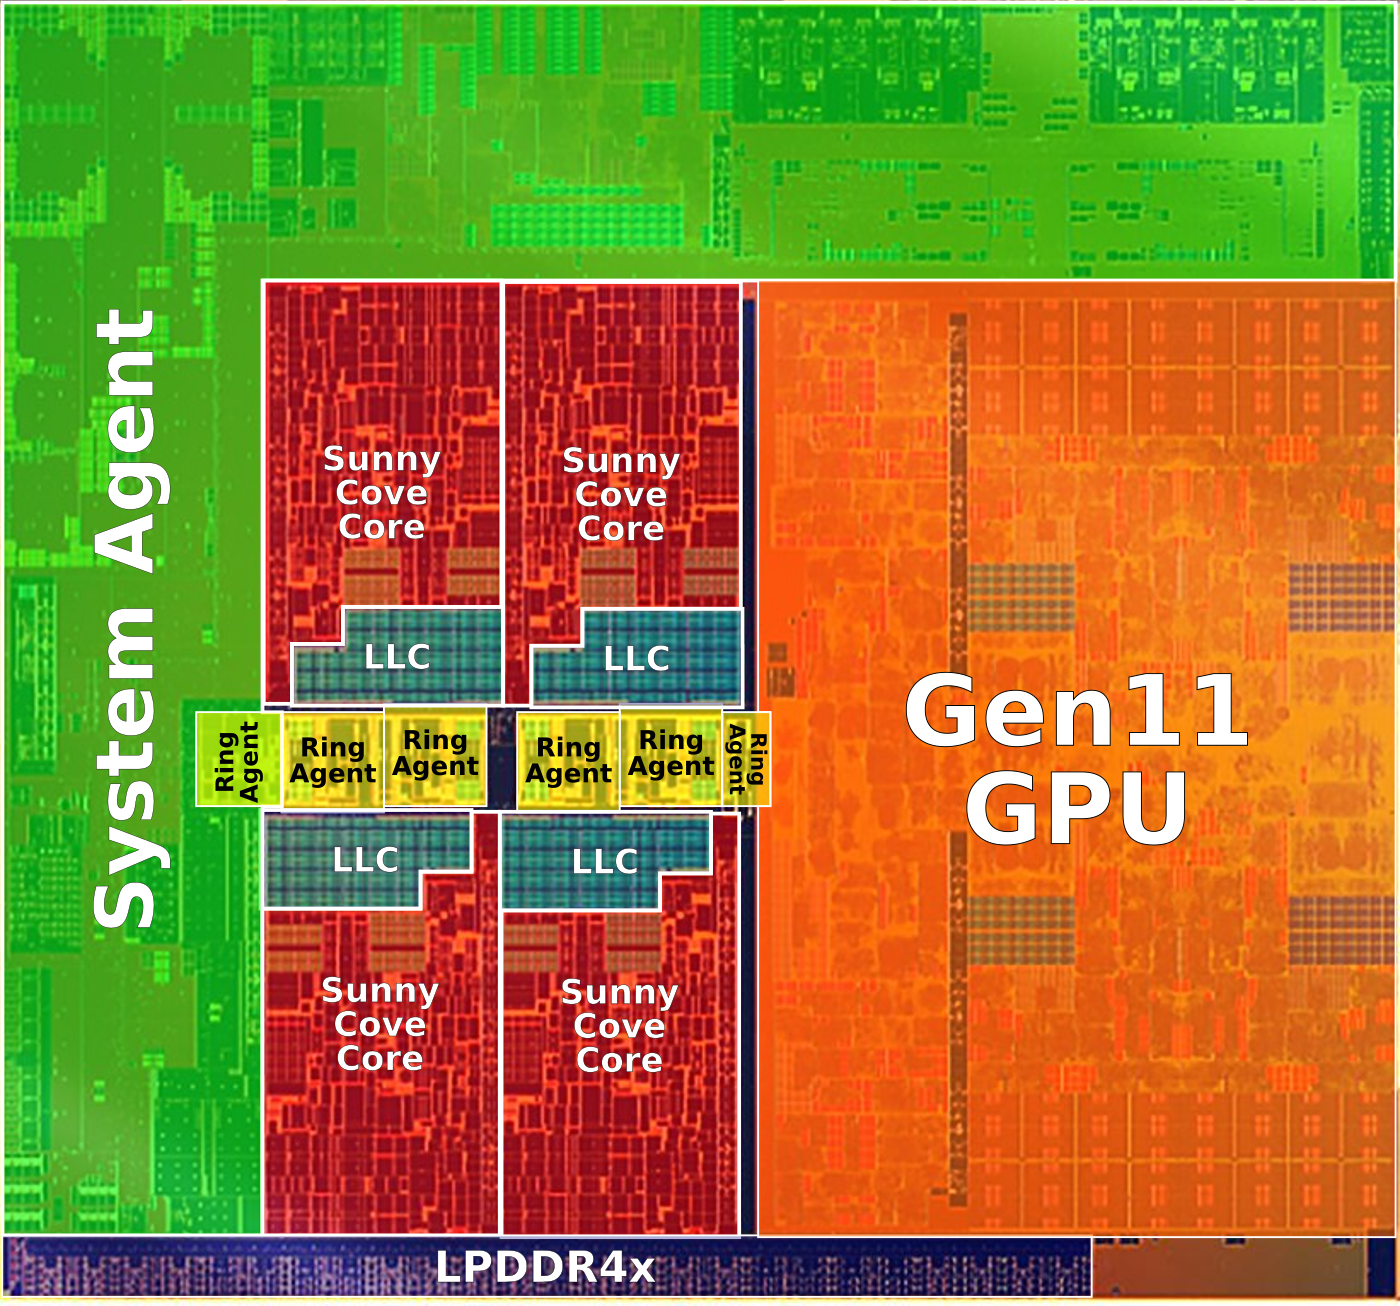
\includegraphics[width=0.3\textwidth]{figures/ice_lake_die_(quad_core)_(annotated)}
  \end{tabular}
  \caption{Over the past fifteen years, the highest-performance computation resources in a mainstream microprocessor have shifted from a small fraction of die area on the CPU to a much larger fraction in an integrated GPU\@. Left: one core of AMD's K8L ``Deerhound'' CPU (2006). Heavy white boxes mark the compute units. Right: Intel Ice Lake hybrid CPU-GPU (2019). Intel's GPU is not only capable of 3D graphics but also general-purpose compute through interfaces like OpenCL\@. \label{fig:gpus-on-modern-processors}} \end{figure}

By focusing on throughput, GPU vendors build designs that are well-suited to address today's most important technology trends. Modern VLSI gives us an increasing number of transistors but little to no increase in clock speeds; GPU vendors have built hardware and software that together scale well with more, rather than faster, hardware resources. The gap (``memory wall'') between processor capability and memory bandwidth continues to grow; throughput-oriented processors like GPUs are designed to amortize increasing memory latency by quickly context-switching to other parallel work. And in a power-constrained world, GPUs have a significant advantage; in his 2010 Supercomputing keynote, Dally cited contemporary figures of 200~pJ/instruction for GPUs and 2~nJ/instruction for CPUs~\cite{Dally:2010:GCT}, with the GPU's power efficiency advantage changing little over the past decade~\cite{Dally:2020:DHA}. It is thus no surprise that even CPU vendors are increasingly emphasizing GPU-like cores on their most recent processors (Figure~\ref{fig:gpus-on-modern-processors}).

With power constraints continuing to be the main bottleneck in increased performance, the superior power-performance of GPUs will make them increasingly attractive. Power constraints are also motivating overprovisioned systems, particularly systems-on-a-chip, where only a subset of the silicon can be powered at any one time~\cite{Esmaeilzadeh:2011:DSA}. Such systems tilt toward more heterogeneity, further motivating hybrid systems---and an increased need for the more energy-efficient GPU-focused computation---as the future norm.
% https://www.nextplatform.com/2022/11/14/testing-the-mettle-of-the-top-supercomputing-iron-on-earth/

But, the front-and-center reason for a continued focus on GPU graph analytics today is outside the scope of graph analytics entirely. The new reality is:

\begin{itemize}
  \item The recent and extremely rapid rise of training deep neural networks for deep-learning applications~\cite{Amodei:2015:DS2,Chetlur:2014:CEP,Coates:2013:DLW,Hannun:2014:DSU}---a field led by NVIDIA GPUs and CUDA---has resulted in NVIDIA-GPU-equipped data centers in nearly every large Internet company and NVIDIA GPUs in each of the three major cloud computing providers. As well, GPUs have made enormous inroads into the largest-scale computations. GPU-centered machines dominate the top of the biannual TOP500 list~\cite{top500:nov2022}, including 7 of the top 10 (\#1 and \#3 have AMD GPUs; 157 total of the 168 GPU-centered machines have NVIDIA GPUs). In systems that have high compute requirements, GPU hardware is now ubiquitous.
  \item Moving data to and from GPUs remains, and appears likely to remain, expensive. Because machine learning and scientific computation are primarily performed today on GPUs, we see an accelerating focus toward ensuring that entire computational pipelines of interest are also on GPUs, to avoid this communication cost. (As an example, it is faster to perform an entire Gunrock breadth-first search on a graph than to transfer that graph between CPU and GPU\@.) So, even if GPU graph applications ran only equally fast as their CPU equivalents, they still offer significant value because they enable faster execution of entire workloads.
\end{itemize}

As a consequence of these two broad trends, NVIDIA has made a large investment into its open-source data science framework, RAPIDS, which has already integrated Gunrock into its codebase and releases, and which will allow us to immediately bring the results from this proposal into widespread use.

\end{comment}



%\rob{One thing that is true, but we're not addressing here --- which may be fine --- is that as fast as we can make the underlying data structures, many tasks may be bottlenecked on system-level limitations like data egress, and file parsing speed; boring but true (see this entire paper on the fact that, with enough cores, parsing the input becomes the limitation for read alignemnt: \url{https://academic.oup.com/bioinformatics/article/35/3/421/5055585}).}
%\mab{this is extremely interesting, but also undermines the message of our proposal. I'm gonna comment out your comment and mine to make the proposal look cleaner.}

%

\textbf{In this project}, we aim to build high-performance and scalable
data-analyses pipelines on the GPU for a wide variety of data-intensive
computations across computational biology, machine learning, databases, and
scientific computing.  To do so, we will address the main computational
bottlenecks that are at the core of many existing systems by developing new
massively parallel and distributed data structures and algorithms for common
and widely-needed data-processing tasks. We aim to address the fundamental
problems described above, \defn{enabling certain heretofore intractable
analyses}, and \defn{vastly reducing (by an order of magnitude or more) the key
computational costs associated with some of the most common data analyses}.    
%
Central to our approach is to leverage the massive parallelism of GPUs. The
challenge with (clusters of) GPUs  is that dynamic data structures have
traditionally  been difficult to design and implement on GPUs, indeed, even on
a single GPU\@. 

We will stress-test our data structural library on computational biology
applications. Specifically, we identify two raw data analysis ``kernels'':
\Kmer analysis and sequence alignment. These kernels are used broadly
throughout computational biology. These are bottlenecks in many
comp.~bio.~workflows, so making them faster and scaling them to larger data
sets will have widespread impact. GPUs offer an avenue to scaling these data
structures. And while GPUs are fast, they are space-constrained.  Therefore,
we need new data structures and algorithms that are space-efficient to speed up
these applications. The scale of comp.~bio.~applications are such that scale
out to multiple, distributed GPUs will be necessary in this setting. See
\Cref{sec:multigpu} for specifics.  




\subsection{Our proposed work}

We believe the answer to these challenges is a collection of  memory-efficient,
high-performance, dynamic, scalable and massively-parallel data structures.
%that can be directly used by computational biology applications. 
Because these data structures are used across multiple applications and domains
we propose to build a \emph{standalone library} comprising these data
structures. A standalone library will enable easy integration and adoption of
these data structures in the applications from this proposal (and many others).

\paragraph{Our approach is four-pronged.}  We will develop new {algorithmic
theory} to design scalable data structures; we will develop new {systems} that
implement our solutions in a scale-up manner,  both on CPU and GPU\@; we will a
develop new framework to distribute our solutions in an {HPC} environment, so
they scale out to clusters of GPUs; and finally we will validate our solutions
on {computational biology} workloads.
%
Specifically, our data structures are: \textbf{filters}, \textbf{hash tables},
\textbf{string indexes}, \textbf{sketches}, and related auxiliary data
structures.  We propose three specific common computational biology analyses on
which we will validate our solutions: {large-scale raw sequence
search},{taxonomic classification for metagenomic data},{pangenomic indexing
and analysis}.   See Section~\ref{sec:compbio} for a description of these
analysitcal pipelines.

\mfc{This needs non-bio applications, I would think}
However, while we will focus and validate on these applications, it is critical
to point out that the data structures, algorithms, and libraries that we build
will find immediate application a much larger array of analyses, some of which
we will endeavour to build ourselves. For example, with the ability to perform
rapid seeding on the GPU (using the indices described herein), and taking
advantage of our own expertise in building computationally efficient tools for
the pre-processing of single-cell sequencing data~\cite{he2022alevin}, we
believe that single-cell RNA-seq preprocessing will be an immediate
``low-hanging'' fruit that can be accelerated with our stack. It has already
been demonstrated by NVIDIA that their RAPIDS single-cell~\cite{rapids} library
can speed up steps of the downstream analysis of single-cell count matrices
from 4.7--850$\times$. Yet, the preprocessing of raw data to obtain the count
matrices to be analyzed, a computationally intensive process, does not yet have
a GPU implementation. However, the required computation is embarrassingly
parallel, with the processing of each sample requiring the alignment of
hundreds of millions to billions of sequencing reads (highly parallelizable),
followed by barcode correction (requires some synchronization) and UMI
resolution (highly parallelizable as each cell can be evaluated independently).
Thus, we anticipate implementing this preprocessing using our GPU-enhanced
stack will see a one to two order-of-magnitude performance improvement over
existing state-of-the-art solutions; a critical necessity given the incredibly
rapid growth of single-cell sequencing data~\cite{scgrowth2022}.

% If successful we will be able to perform complex data analyses to answer biological questions on available terabyte- and petabyte-scale datasets, for example, raw sequencing data from SRA~\cite{kodama2012sequence}, metagenomic data from WA and Rhizo~\cite{hofmeyr2020terabase}, and pangenomic data from 100,000 genome project~\cite{1002021100}. \john{These cites / this argument is also made a page earlier; consider deleting this.} Existing data structures and software tools fail to scale to these data sizes, making these publicly available and highly valuable data resources largely inert.


\mfc{this feels apologetic.  Is there a better title that project's novelties?}
\textbf{The project’s novelties are: a vertical-stack approach} spanning
\textbf{theory and algorithms} (highly concurrent, dynamic, and distributed
data structures); \textbf{systems} (scaling up using GPU acceleration);
\textbf{high-performance computing} (scaling out using distributed data
structures); and \textbf{applications} (computational biology applications);
new parallel and distributed data structures and algorithms to exploit the
massive compute on GPUs that can be applicable to other application domains;
and an API for developers to quickly and seamlessly integrate high-performance
and scalable data structures in applications.
%
Our team includes a highly interdisciplinary team of researchers across four
focus areas: applications (computational biology), theory and algorithms,
systems, and high-performance computing. The team is taking a holistic
theory/systems/HPC/applications co-design approach to explore four tightly
interconnected research modules. These research modules are structured from
bottom-up across the computing stack.

% \prashant{Add a brief application about Single cell as another application of the library.}

% \subsection{Cross-cutting concerns}

% The cross-cutting concerns of particular interest to the PPoSS program are well-covered by this proposal.

% \begin{description}%[noitemsep,nolistsep]
%   \item[Scalability and performance] are our main evaluation criteria. Our explicit goals are to both increase the performance of our target applications on existing datasets and to increase the scale of datasets we can target beyond what is currently possible.

%   \item[Correctness and accuracy] are primary targets of our software development methodology (Section~\ref{sec:sw-methodology}), which describes our proposed use a suite of functional and performance tests; use of code-coverage tools together with these tests; and the use of continuous-integration and continuous-development tools and methodologies.

%   \item[The capabilities of heterogeneous architectures] are our chief motivation for our choice of single-GPU, multi-GPU, and multi-node-multi-GPU architectural targets for this work. We elaborate on this choice in Section~\ref{sec:gpu}.


%\end{description}


